\documentclass[11pt,a4paper, dvipdfmx]{jsarticle}
\usepackage{amsmath,amssymb}
\usepackage{amsthm}
\usepackage{ascmac}
\usepackage{bm}
\usepackage[dvipdfmx]{graphicx}	% required for `\includegraphics' (yatex added)
\usepackage{setspace}           % required for `\doublespace'
\usepackage{tikz}
\usepackage{tikz-cd}
\usetikzlibrary{angles, positioning, shapes, arrows.meta, decorations.pathmorphing}
%\usetikzlibrary{intersections, calc, arrows, positioning, arrows.meta}
\usepackage{tcolorbox}  % 定理環境の装飾
\tcbuselibrary{skins, breakable, theorems}
\usepackage{xcolor}
\usepackage{natbib}
\usepackage{pxrubrica}
\usepackage[margin=30truemm, left=40truemm, right=40truemm]{geometry}
\usepackage{thmbox}     % required for theorem environment with side bar
%
\setlength{\parskip}{3mm} %段落間にスペースを入れる


% \pagestyle{myheadings}
% \markright{\footnotesize \sf 2022秋期「哲学者のための数学」授業資料(大塚淳) \ \ 配布禁止}


\theoremstyle{definition}
\newtheorem[S]{exercise}{練習問題}[section]
\newtheorem[S]{example}{事例}[section]
\newtheorem[S]{fact}{事実}[section]
\newtheorem[S]{attn}{注意}[section]
\newtheorem[S]{develop}{発展}[section]
\renewcommand{\theattn}{}

\newtcbtheorem[auto counter, number within=section]{rei}{事例}{
    breakable,
    coltitle=black,
    fonttitle=\bfseries,
    enhanced, colback=white, frame hidden, borderline west = {0.5pt}{5pt}{black},
%    number freestyle={\noexpand\thesection.\noexpand\arabic{\tcbcounter}}
}{rei}

\newtcbtheorem[auto counter, number within=section]{prop}{命題}{
    breakable,
    coltitle=black,
    fonttitle=\bfseries,
    enhanced, colback=white, frame hidden, borderline west = {0.5pt}{5pt}{black},
%    number freestyle={\noexpand\thesection.\noexpand\arabic{\tcbcounter}}
}{prop}

\newtcbtheorem[number within=section]{renshu}{練習問題}{
    breakable,
    coltitle=black,
    fonttitle=\bfseries,
    enhanced, colback=white, frame hidden, borderline west = {0.5pt}{5pt}{black}
}{renshu}


\newtcbtheorem[number within=section]{hatten}{発展}{
    breakable,
    coltitle=black,
    fonttitle=\bfseries,
    enhanced, colback=white, frame hidden, borderline west = {0.5pt}{5pt}{black}
}{renshu}


\newtcbtheorem[number within=section]{dfn}{定義}{
    fonttitle=\bfseries,
    enhanced, colback=white
}{dfn}


% Bold face capital letters:
\newcommand{\bfzero}{\boldsymbol{0}}
\newcommand{\bfone}{\boldsymbol{1}}
\newcommand{\bfA}{\boldsymbol{A}}
\newcommand{\bfB}{\boldsymbol{B}}
\newcommand{\bfC}{\boldsymbol{C}}
\newcommand{\bfD}{\boldsymbol{D}}
\newcommand{\bfE}{\boldsymbol{E}}
\newcommand{\bfF}{\boldsymbol{F}}
\newcommand{\bfG}{\boldsymbol{G}}
\newcommand{\bfH}{\boldsymbol{H}}
\newcommand{\bfI}{\boldsymbol{I}}
\newcommand{\bfJ}{\boldsymbol{J}}
\newcommand{\bfK}{\boldsymbol{K}}
\newcommand{\bfL}{\boldsymbol{L}}
\newcommand{\bfM}{\boldsymbol{M}}
\newcommand{\bfN}{\boldsymbol{N}}
\newcommand{\bfO}{\boldsymbol{O}}
\newcommand{\bfP}{\boldsymbol{P}}
\newcommand{\bfQ}{\boldsymbol{Q}}
\newcommand{\bfR}{\boldsymbol{R}}
\newcommand{\bfS}{\boldsymbol{S}}
\newcommand{\bfT}{\boldsymbol{T}}
\newcommand{\bfU}{\boldsymbol{U}}
\newcommand{\bfV}{\boldsymbol{V}}
\newcommand{\bfW}{\boldsymbol{W}}
\newcommand{\bfX}{\boldsymbol{X}}
\newcommand{\bfY}{\boldsymbol{Y}}
\newcommand{\bfZ}{\boldsymbol{Z}}

\newcommand{\bfa}{\boldsymbol{a}}
\newcommand{\bfb}{\boldsymbol{b}}
\newcommand{\bfc}{\boldsymbol{c}}
\newcommand{\bfd}{\boldsymbol{d}}
\newcommand{\bfe}{\boldsymbol{e}}
\newcommand{\bff}{\boldsymbol{f}}
\newcommand{\bfk}{\boldsymbol{k}}
\newcommand{\bfm}{\boldsymbol{m}}
\newcommand{\bfn}{\boldsymbol{n}}
\newcommand{\bfo}{\boldsymbol{o}}
\newcommand{\bfp}{\boldsymbol{p}}
\newcommand{\bfq}{\boldsymbol{q}}
\newcommand{\bfr}{\boldsymbol{r}}
\newcommand{\bfs}{\boldsymbol{s}}
\newcommand{\bft}{\boldsymbol{t}}
\newcommand{\bfu}{\boldsymbol{u}}
\newcommand{\bfv}{\boldsymbol{v}}
\newcommand{\bfw}{\boldsymbol{w}}
\newcommand{\bfx}{\boldsymbol{x}}
\newcommand{\bfy}{\boldsymbol{y}}
\newcommand{\bfz}{\boldsymbol{z}}



% BB (???) capital letters:
\newcommand{\bbA}{\mathbb{A}}
\newcommand{\bbB}{\mathbb{B}}
\newcommand{\bbC}{\mathbb{C}}
\newcommand{\bbD}{\mathbb{D}}
\newcommand{\bbE}{\mathbb{E}}
\newcommand{\bbF}{\mathbb{F}}
\newcommand{\bbG}{\mathbb{G}}
\newcommand{\bbI}{\mathbb{I}}
\newcommand{\bbN}{\mathbb{N}}
\newcommand{\bbP}{\mathbb{P}}
\newcommand{\bbQ}{\mathbb{Q}}
\newcommand{\bbR}{\mathbb{R}}
\newcommand{\bbU}{\mathbb{U}}
\newcommand{\bbV}{\mathbb{V}}
\newcommand{\bbX}{\mathbb{X}}
\newcommand{\bbY}{\mathbb{Y}}
\newcommand{\bbZ}{\mathbb{Z}}
\newcommand{\bbone}{{\ifmmode\mathrm{1\!l}\else\mbox{\(\mathrm{1\!l}\)}\fi}}


% Caligraphic math capital letters:
\newcommand{\mcalA}{\mathcal{A}}
\newcommand{\mcalB}{\mathcal{B}}
\newcommand{\mcalC}{\mathcal{C}}
\newcommand{\mcalD}{\mathcal{D}}
\newcommand{\mcalE}{\mathcal{E}}
\newcommand{\mcalF}{\mathcal{F}}
\newcommand{\mcalG}{\mathcal{G}}
\newcommand{\mcalH}{\mathcal{H}}
\newcommand{\mcalI}{\mathcal{I}}
\newcommand{\mcalJ}{\mathcal{J}}
\newcommand{\mcalK}{\mathcal{K}}
\newcommand{\mcalL}{\mathcal{L}}
\newcommand{\mcalM}{\mathcal{M}}
\newcommand{\mcalN}{\mathcal{N}}
\newcommand{\mcalO}{\mathcal{O}}
\newcommand{\mcalP}{\mathcal{P}}
\newcommand{\mcalQ}{\mathcal{Q}}
\newcommand{\mcalS}{\mathcal{S}}
\newcommand{\mcalT}{\mathcal{T}}
\newcommand{\mcalU}{\mathcal{U}}
\newcommand{\mcalV}{\mathcal{V}}
\newcommand{\mcalX}{\mathcal{X}}
\newcommand{\mcalY}{\mathcal{Y}}
\newcommand{\mcalZ}{\mathcal{Z}}

% Graph nodes notations:
\newcommand{\PA}{\mathit{PA}}
\newcommand{\bfPA}{\mathbf{PA}}
\newcommand{\CH}{\mathit{CH}}
\newcommand{\bfCH}{\mathbf{CH}}
\newcommand{\DS}{\mathit{DS}}
\newcommand{\bfDS}{\mathbf{DS}}
\newcommand{\ND}{\mathit{ND}}
\newcommand{\bfND}{\mathbf{ND}}
\newcommand{\AN}{\mathit{an}}
\newcommand{\bfAN}{\mathbf{an}}
\newcommand{\pa}{\mathit{pa}}
\newcommand{\bfpa}{\mathbf{pa}}
\newcommand{\ch}{\mathit{ch}}
\newcommand{\bfch}{\mathbf{ch}}
\newcommand{\ds}{\mathit{ds}}
\newcommand{\bfds}{\mathbf{ds}}
\newcommand{\nd}{\mathit{nd}}
\newcommand{\bfnd}{\mathbf{nd}}
\newcommand{\an}{\mathit{an}}
\newcommand{\bfan}{\mathbf{an}}



\DeclareMathOperator*{\argmax}{arg\,max}
\DeclareMathOperator*{\argmin}{arg\,min}
\DeclareMathOperator*{\argsup}{arg\,sup}
\DeclareMathOperator*{\arginf}{arg\,inf}
\DeclareMathOperator{\erfc}{erfc}
\DeclareMathOperator{\diag}{diag}
\DeclareMathOperator{\cum}{cum}
\DeclareMathOperator{\sgn}{sgn}
\DeclareMathOperator{\tr}{tr}
\DeclareMathOperator{\spn}{span}
\DeclareMathOperator{\adj}{adj}
\DeclareMathOperator{\E}{\mathbb{E}}
\DeclareMathOperator{\var}{Var}
\DeclareMathOperator{\cov}{Cov}
\DeclareMathOperator{\corr}{corr}
\DeclareMathOperator{\sech}{sech}
\DeclareMathOperator{\sinc}{sinc}
\DeclareMathOperator*{\lms}{l.i.m.\,}
\newcommand{\varop}[1]{\var\left[{#1}\right]}
\newcommand{\covop}[2]{\cov\left({#1},{#2}\right)}
\newcommand{\T}{^\textrm{T}}
\newcommand\indep{\protect\mathpalette{\protect\independenT}{\perp}}
\def\independenT#1#2{\mathrel{\rlap{$#1#2$}\mkern2mu{#1#2}}}

\newcommand{\bfalpha}{\boldsymbol{\alpha}}
\newcommand{\bfbeta} {\boldsymbol{\beta}}
\newcommand{\bfgamma}{\boldsymbol{\gamma}}
\newcommand{\bfeta}  {\boldsymbol{\eta}}
\newcommand{\bftheta}{\boldsymbol{\theta}}
\newcommand{\bflambda}   {\boldsymbol{\lambda}}
\newcommand{\bfmu}   {\boldsymbol{\mu}}
\newcommand{\bfnu}   {\boldsymbol{\nu}}
\newcommand{\bfxi}   {\boldsymbol{\xi}}
\newcommand{\bfpsi}  {\boldsymbol{\psi}}
\newcommand{\bfphi}   {\boldsymbol{\phi}}
\newcommand{\bfrho}   {\boldsymbol{\rho}}
\newcommand{\bfvarepsilon}{\boldsymbol{\varepsilon}}
%\newcommand{\qed}{{qed}}
%\newcommand{\eqalignno}[1]{\begin{array}{ccccccc}#1\end{array}}

\newcommand{\bfGamma}{\boldsymbol{\Gamma}}
\newcommand{\bfTheta}{\boldsymbol{\Theta}}
\newcommand{\bfLambda}   {\boldsymbol{\Lambda}}
\newcommand{\bfPsi}  {\boldsymbol{\Psi}}
\newcommand{\bfPhi}   {\boldsymbol{\Phi}}
\newcommand{\bfSigma}  {\boldsymbol{\Sigma}}
\newcommand{\bfOmega}  {\boldsymbol{\Omega}}


% DISTRIBUTIOoNS: 
\newcommand{\normal}{\mathcal{N}}
\newcommand{\binomial}{\mathcal{B}}
\newcommand{\multinomial}{\mathcal{M}}
\newcommand{\exponential}{\mathcal{E}}
\newcommand{\geometric}{\mathcal{G}}
\newcommand{\poisson}{\mbox{Poisson}}
\newcommand{\uniform}{\mbox{Uniform}}

% Logic
\newcommand{\true}{\texttt{true}}
\newcommand{\false}{\texttt{false}}


%PSTricks (commande for latent nodes)
\newcommand{\lnode}[4]{ \cnode(#1){#2}{#3}\rput(#1){\footnotesize#4} }

% KEEPING TRACK OF WORK
\newcommand{\todo}[1]
{
{\color{red}{
[TODO: #1]}}
\addcontentsline{toc}{subsection}{TO DO: #1}
}

\newcommand{\fixme}[1]{{\color{red}{#1}}}

\newenvironment{answer}[1]
{\par \color{blue}{#1}}
{}


\newcommand{\note}[2]
{
{\color{red}{
[#1: #2]}}
}




\makeatletter
% define \citepos for posesive citation (e.g. Otsuka's (2015))
\DeclareRobustCommand\citepos
  {\begingroup
   \let\NAT@nmfmt\NAT@posfmt% ...except with a different name format
   \NAT@swafalse\let\NAT@ctype\z@\NAT@partrue
   \@ifstar{\NAT@fulltrue\NAT@citetp}{\NAT@fullfalse\NAT@citetp}}

\let\NAT@orig@nmfmt\NAT@nmfmt
\def\NAT@posfmt#1{\NAT@orig@nmfmt{#1's}}
\makeatother




% Code for drawing color circle used in topology (pathconnectedness)
\usepackage{xparse}
\ExplSyntaxOn

\keys_define:nn { colour_transition_circle } {
    inner   .fp_set:N   = \l__inner_radius,
    inner   .initial:n  = {2},
    outer   .fp_set:N   = \l__outer_radius,
    outer   .initial:n  = {3},
    angle   .fp_set:N   = \l__start_angle,
    angle   .initial:n  = {0}
}

\NewDocumentCommand \ColourTransitionCircle { O{} m } {
\group_begin:
    \keys_set:nn { colour_transition_circle } {#1}
    \clist_clear:N \l_tmpa_clist
    \clist_map_inline:nn {#2} {
        \clist_put_right:Nn \l_tmpa_clist {##1}
        %\clist_put_right:Nn \l_tmpa_clist {##1}
    }
    \exp_args:Nx \col_trans_circ:n \l_tmpa_clist
\group_end:
}

\cs_new_protected:Npn \col_trans_circ:n #1 {
    \int_step_inline:nnnn {1} {1} {\clist_count:n {#1} - 1} {
        \path[top~color=\clist_item:nn {#1} {##1}, bottom~color=\clist_item:nn {#1} {##1+1}, shading~angle={270-(180-360/\clist_count:n {#1})/2+(##1-1)*360/\clist_count:n {#1}+\fp_use:N \l__start_angle}] ({\fp_use:N \l__inner_radius*cos((##1-1)*360/\clist_count:n {#1}+\fp_use:N \l__start_angle)},{\fp_use:N \l__inner_radius*sin((##1-1)*360/\clist_count:n {#1}+\fp_use:N \l__start_angle)}) arc[radius = \fp_use:N \l__inner_radius, start~angle={(##1-1)*360/\clist_count:n {#1}+\fp_use:N \l__start_angle}, delta~angle=360/\clist_count:n {#1}] -- ({\fp_use:N \l__outer_radius*cos(##1*360/\clist_count:n {#1}+\fp_use:N \l__start_angle)},{\fp_use:N \l__outer_radius*sin(##1*360/\clist_count:n {#1}+\fp_use:N \l__start_angle)}) arc[radius = \fp_use:N \l__outer_radius, start~angle={##1*360/\clist_count:n {#1}+\fp_use:N \l__start_angle}, delta~angle=-360/\clist_count:n {#1}] -- cycle;
    }
    \path[top~color=\clist_item:nn {#1} {\clist_count:n {#1}}, bottom~color=\clist_item:nn {#1} {1}, shading~angle={180-180/\clist_count:n {#1}+\fp_use:N \l__start_angle}]({\fp_use:N \l__inner_radius*cos((\clist_count:n {#1}-1)*360/\clist_count:n {#1}+\fp_use:N \l__start_angle)},{\fp_use:N \l__inner_radius*sin((\clist_count:n {#1}-1)*360/\clist_count:n {#1}+\fp_use:N \l__start_angle)}) arc[radius = \fp_use:N \l__inner_radius, start~angle={(\clist_count:n {#1}-1)*360/\clist_count:n {#1}+\fp_use:N \l__start_angle}, delta~angle=360/\clist_count:n {#1}] -- ({\fp_use:N \l__outer_radius*cos(\clist_count:n {#1}*360/\clist_count:n {#1}+\fp_use:N \l__start_angle)},{\fp_use:N \l__outer_radius*sin(\clist_count:n {#1}*360/\clist_count:n {#1}+\fp_use:N \l__start_angle)}) arc[radius = \fp_use:N \l__outer_radius, start~angle={\clist_count:n {#1}*360/\clist_count:n {#1}+\fp_use:N \l__start_angle}, delta~angle=-360/\clist_count:n {#1}] -- cycle;
}

\ExplSyntaxOff


\usepackage{tikz}
\usetikzlibrary{intersections, calc, arrows, positioning, arrows.meta}

\begin{document}


\title{6. モノイド}
\author{2023秋期「哲学者のための数学」授業資料(大塚淳)}
\date{ver. \today}
\maketitle

\section{モノイドとは何か,なぜそれを学ぶのか}
前章で見た位相は,空間に関する幾何学的な概念であった.
一方本章および次章の主題となるモノイドや群は,本質的に代数的な「計算」にまつわる概念である.
よって我々は,代数,幾何と来て再び代数の世界に戻ってきた.

文系の学生にとって,「位相」という言葉は耳にしたことくらいはあっても,「モノイド」となると聞いたこともない,という人も多いかもしれない.
しかし実のところ我々は皆,小学生のころからモノイドに親しんでいる.
というのも,足し算や掛け算などはまさにこのモノイドの作用に他ならないからだ.
モノイド(や次の章で扱う群)は,そうした四則演算を始めとした「演算」一般の最もプリミティブな形を抜き出したものと言える.
しかしながら,モノイドを数学を超えた自然科学一般において極めて重要なものにしているのは,それが対象や系の変化・発展を表すための非常に自然な枠組みを提供する,という点である.
もちろん,哲学もそれに無縁ではない.というのも,そこには法則や自由,決定論,目的論など,様々な哲学的な含意が含まれているからだ.

このようにモノイドの応用は多岐にわたるが,その基本的な考え方はこれ以上ないくらいシンプルである.
ここではその本質的な点のみに的を絞って紹介したい.
そこから得られるモノイドは,数学者や物理学者からしたらおもちゃみたいに簡単なものでしかないかもしれないが,その哲学的含意を考えるには十分であろう.

\section{モノイド}
まずはいつものように,集合をベースにモノイドを定義しよう.

\begin{dfn}{モノイド}
集合$M$上に,積と呼ばれる二項写像$\circ: M \times M \to M$が定義されており,以下の条件を満たすとき,組$(M, \circ, i)$を\emph{モノイド}(monoid)という.
\begin{enumerate}
 \item $M$の任意の元$l, m, n$に対して,結合律$(l \circ m) \circ n = l \circ (m \circ n)$がなりたつ.
 \item \emph{単位元}(identity element)と呼ばれる元$i \in M$が存在して,$M$の任意の元$m$に対して,$i \circ m = m \circ i = m$がなりたつ.
\end{enumerate} 
\end{dfn}

これだけである.
つまりモノイドとは,その2つの元$m,n$をある元$m \circ n$に対応させるモノイド演算$\circ$が備わっているような集合である.
公理1は,この演算が結合律を満たすこと,そして公理2はこの演算において「何もしない」単位元が存在することを言っている.
しばしば演算記号は省略され,$m \circ n$は$mn$のように書かれる.
また誤解が生じないときは,演算や単位元を明示せずに単に$M$がモノイドである,というように言うこともある.


\begin{rei}{}{n_monoid}
ゼロを含む自然数$\bbN$(つまり非負整数)は,二項演算$+$とモノイドをなす.ここでの単位元は$0$である.
実際任意の自然数$x, y, z$について,$(x+y)+z = x + (y+z)$かつ$0 + x = x + 0 = x$. 
同様に,$\bbN$が乗算$\times$についてもモノイドとなることを確認せよ(その単位元はなんだろうか).
%また明らかなように,上の議論は自然数の代わりに有理数$\bbQ$,実数$\bbR$のゼロ以上の部分を用いても成立する.
\end{rei}

\begin{rei}{}{r_monoid}
足し算についての上の議論は,自然数の代わりに有理数$\bbQ$,実数$\bbR$のゼロ以上の部分を用いても成立する.
例えば$\bbR^+ := \{ x \in \bbR | x \geq 0 \}$と定義すると,$(\bbR^+, +, 0)$はモノイドである.
(負の部分はどうなるのか,と思うかもしれないが,これはあとで群を定義するときに見る.)
\end{rei}

モノイドの演算が具体的にどうなっているのかは,それぞれの元のペアの演算結果を明示することによって表示できる.
例えば,お馴染みの「九九の表」は,自然数の掛け算モノイドの演算を表で表したものだ:
\[
\begin{array}{c|cccccc}
       & 1 & 2 & 3 & \dots & n & \dots \\ \hline
     1 & 1 & 2 & 3 & \dots & n & \dots \\ 
     2 & 2 & 4 & 6 & \dots & 2n & \dots \\ 
     3 & 3 & 6 & 9 & \dots & 3n & \dots \\ 
     \vdots & \vdots & \vdots & \vdots & & \vdots & \\
     m & m & m2 & m3 & \cdots & mn & \cdots \\
     \vdots & \vdots & \vdots & \vdots & & \vdots & \\
\end{array}
\]
九九表の各マスは,モノイド$(\bbN, \times, 1)$の1から9までの各元(一番左の列)が,それぞれ1から9までの元(一番上の行)をどの自然数に対応させるかを表している.
すべてのモノイド演算は,原理的にこうした表(「積表」という)によって表すことができる.
つまり我々は小学生のころからモノイドを知っていたのである!


\begin{hatten}{実数の様々な側面}{reals}
我々は今まで,(非負)実数$\bbR$を様々な数学的構造として見てきた.
まず2章ではそれが非可算無限集合であることを確認した.
3章ではその要素の間に大小関係$\leq, \geq$を入れた全順序集合として見た.
4章では,実数を開区間$(a,b)$からなる開集合を持つ位相空間として特徴づけた.
そしてここでは,二項演算$+$および$\times$が定義されたモノイドとして定義した.
このように,同じ「実数の集合」でも様々な顔を持ち,それらの顔はすでに見たような公理によって構成される.
我々が普段何気なく使う実数は,実はこうした顔全てをあわせもつ存在なのである.

 もちろん,実数の特徴づけはこれで終わりなわけではない.
 まず引き算と割り算の導入がまだであるし(これは以下で群のところで見る),またここで導入した足し算と掛け算が互いにどう関係し合うのか(例えば分配法則$a(b+c) = ab + ac$が満たされるか)などは,別個の公理によって定めなければならない.
 このためにはさらに\emph{環}(ring),\emph{体}(field)といった概念を導入しなければならいのだが,本授業ではそこまでは扱わない.
\end{hatten}

モノイドの例は数学以外にも事欠かない.
対象を繋げたり,行為を続けて行ったりというような逐次的なプロセスは,自然にモノイド構造を生み出す.

\begin{rei}{自由モノイド}{free_monoid}
3つの記号$a, b, c$に空文字$i$を加えた集合を$\Sigma = \{a, b, c, i \}$とする.
これらの文字(列)を横に繋げたものを積で表す(e.g. $a \circ b = ab, aabc \circ bac = aabcbac$).
$i$は空文字なので繋げても何も変化しないとする(e.g. $ai = ia = a$).
積による合成を再帰的に繰り返すことで,無限に文字列を生成することができる.
このように生成された文字列の集合を$\Sigma_*$とすると,これは$\circ$を積,$i$を単位元としたモノイドになっており,これを$\Sigma$上に生成される\emph{自由モノイド}(free monoid)という.
「消去(backspace)」を使わずにパソコンのキーストロークによって得られる文は,こうした自由モノイドの一例である.
\end{rei}

この例では,上の自然数の例とは異なり,有限個の「素材」$\Sigma$を元手として,それを積で合成することで$\Sigma_*$における無数のモノイド元を生成している.
生成されたモノイドが自由であるとは,それらの元の間に自明でないような等号関係がない,ということを意味している.
実際,上の$\Sigma_*$においては,いかなる文字列もそれ自身以外とは等しくない.
一方自然数のほうは,例えば$7 + 5 = 2 + 10 = 12$のように,複数の元の間に等号関係がある.


\begin{rei}{ロボットのプログラム}{robot_program}
プログラムによって操作できるロボットを考える.
ロボットに可能な動きは一歩前進する($a$)・右を向く($b$)・左を向く($c$)・何もしない($i$)の4つとする.
プログラムはこれら可能な4つの動作を有限回繰り返したものとして書かれる.
例えば$aaba$を入力すると,ロボットは前に二歩進んだあと右に一歩進む.
任意のプログラムは逐次的につなげることができる.例えば$aaba \circ cica$は$cica$を実行した後に$aaba$を実行する.
このロボットのプログラムは,上と同じようにモノイド$\Sigma_*$を生成する.
\end{rei}

これは前の事例\ref{rei:free_monoid}と構造上ほぼ同じように見えるが,重要な違いがある.
事例\ref{rei:free_monoid}の記号連結は自由モノイドを生成した.
一方,ロボットのプログラムの方はどうであろうか.
確かに,$bcaa$は前に二歩進んで左・右,$aabc$は左・右を向いてから前に二歩,とロボットの動作としては異なる.
その意味において,ロボットの\emph{動作}のプログラムとしてはこちらも自由モノイドである.
しかし,プログラムの最終的な\emph{結果}にだけ着目すると,両者とも同じ,単に前に二歩進む($aa$)のと同じ結果をもたらす.
よって結果の観点からは$bcaa = aabc = aa$というような等号関係が成立する.
その意味では,このモノイドには単に動作を組み合わせてできる様々なプログラムが含まれているだけでなく,それらのプログラムの間の等号関係を含んでいる.
よってここでの$\Sigma_*$は基本動作の集合から生成されたモノイドではあるが,自由に生成されたものではない.



\begin{rei}{人生}{life_monoid}
    我々の人生は選択の連続である.
    毎日の行動の選択肢を$(p)$ 遊ぶ,$(s)$勉強する,$(w)$バイトに行く,$(r)$休むとし,これに名目的な単位元($i$)を加えたものを$M$とする.
    行動$m$をした翌日に$n$を行うことを積$n \circ m$で表すと,$M$はモノイドとなる.
    例えば$prwpssp$は遊び・勉強・勉強・遊び・バイト・休み・遊びの順で過ごした一週間を表している.
    人生は上述の選択肢$M$から生成されるモノイドである.
\end{rei}

この事例は,人生が日々の限られた選択から生成されていく様子をモデル化している.
これは自由モノイドだろうか?
自由モノイドであれば,事例\ref{rei:free_monoid}で一度繋げた文字が取り消せなかったように,一回した選択は取り消しができない,つまり過去を変えることはできない.
一方,自由モノイドでなければ,過去の挽回が可能である.
例えば$ssp = s$という関係性(これは上のモノイドとは別の公理として導入されることになる)は,一日遊んだ後に二日続けて勉強すればそれを帳消しにできる,ということを述べている.

ここではさしあたり,人生とは自由モノイドであると仮定しよう.
今,月曜から木曜までを$rppp$と遊び呆けて過ごしたとする.
このとき,どのように残りを過ごしても,月曜日に遊びに行った事実は変えられない,つまりここから$rpps$という「人生」には到達できない.
ここから,自由モノイドには「元$m$は元$n$から生成可能である」という半順序$n \preceq m$が定義できることがわかる(これが半順序であることを確認せよ).
この半順序は図\ref{fig:monoid_tree}のような木構造をなす(ここではスペースの制約のため「遊ぶ」と「勉強」という二つの選択肢のみを描いている).
この木構造は,自由モノイドによって生成される可能性の一つ一つを,根本から葉先まで続く一本の枝として表している.

\begin{figure}[h]
    \centering
    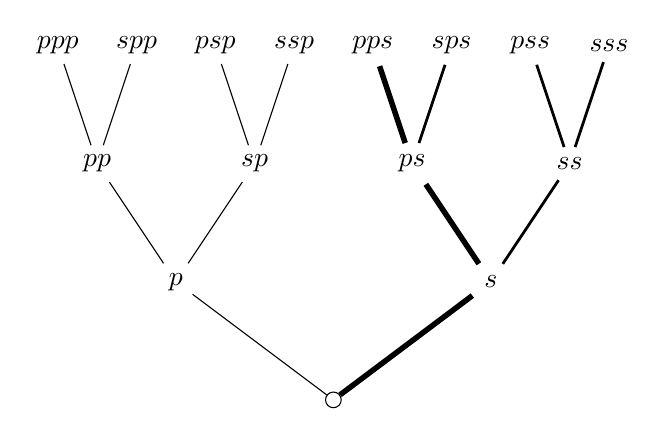
\begin{tikzpicture}[
        grow'=up,
        level 1/.style={sibling distance=4cm},
        level 2/.style={sibling distance=2cm},
        level 3/.style={sibling distance=1cm}
      ]
      
      \node[circle, draw, fill=white, inner sep=2pt] {}
        child {node {$p$}
          child {node {$pp$}
            child {node {$ppp$}}
            child {node {$spp$}}
          }
          child {node {$sp$}
            child {node {$psp$}}
            child {node {$ssp$}}
          }
        }
        child[line width=2pt]  {node {$s$}
          child[line width=2pt] {node {$ps$}
            child {node {$pps$}}
            child[line width=1pt] {node {$sps$}}
          }
          child[line width=1pt]  {node {$ss$}
            child {node {$pss$}}
            child {node {$sss$}}
          }
        };
      \end{tikzpicture}
      \caption{人生モノイドに対応する半順序.ここではスペースの制約のため,選択$p, s$のみを考慮し,3日間のみの分岐を表している.それぞれの枝は異なった「3日分の過ごし方」を表している.太線は遊び・勉強・勉強と過ごした3日間である.2日目の$ps$の時点で,他の6つの可能性は閉ざされている.}
      \label{fig:monoid_tree}
\end{figure}

\begin{renshu}{}{}
    上では人生を自由モノイドとしてしまったが,それは本当にそうなのだろうか.
    自由モノイドでない人生モデルは,人生をどのようなものとして捉えることになるだろうか.
    またそのとき,上で定義した生成可能関係は半順序をなすだろうか.
\end{renshu}    


\section{可換性}
上で見てきたようにモノイドには様々なものがあるが,その中で一番重要な区分は,それが可換であるか否か,というものである.
モノイド$M$が\emph{可換}(commutative)であるとは,その積の結果が順序によらないこと,つまり任意の2つのモノイド元$m,n \in M$について$m \circ n = n \circ m$がなりたつことをいう.
そうならないものが一例でもあるときは,非可換(noncommutative)であるという.

\begin{rei}{}{}
    足し算や掛け算は可換性が満たされる典型例である(任意の数につき$m+n = n+m, m\cdot n = n\cdot m$).
    一方,$n \times n$行列の集合は行列積と単位行列$I$によりモノイドをなすが,これは可換性を満たさない(2つの行列$A, B$について一般に$AB \neq BA$).
\end{rei}


足し算や掛け算に慣れ親しんだ身には,可換性は極めて一般的な性質に映るかもしれない.
しかし上述の定義の通り,それは非常に強い性質である.
モノイドとして表されるような現実世界の「作用」に目を向けると,多くの場面において可換性は必ずしも成立しない.
例えば上の事例で見た自由モノイドによる記号列の生成(\ref{rei:free_monoid})やロボットのプログラム(\ref{rei:robot_program})は明らかに非可換である.
非可換性を証明するためには,モノイド元のうち,$m \circ n \neq n \circ m$であるようなものを一組でも見つければ良い.


\begin{rei}{}{}
    ある人の心に生じる様々な心的刺激の集合を$M$で表すと,これはモノイドを生成する.その元は特定の質を持つ心的刺激,例えば「痛み($m$)」や「熱さ($n$)」であり,単位元は無刺激,積による合成 $m \circ n$ は熱さの後に痛みを感じることである.
    このとき,$M$は明らかに可換ではないだろう.というのも,痛みを感じてから熱さ感じることと,その逆とは明らかに別の感覚刺激だからだ.
\end{rei}

\begin{renshu}{}{}
    事例\ref{rei:life_monoid}の人生モノイドは可換だろうか,非可換だろうか.理由も含めて考えよ.
\end{renshu}

\begin{renshu}{}{}
 全体として非可換なモノイドであっても,特定の元の積では可換性が満たされうる.事例\ref{rei:robot_program}において,その実行結果(動作ではなく)が(i)非可換,(ii)可換となるようなプログラム元のペアをそれぞれ挙げよ.
\end{renshu}

\begin{renshu}{}{}    
    数学以外の事例で,可換/非可換モノイドによってモデル化できそうな現象をそれぞれ一つ挙げよ.その場合の合成と単位元がそれぞれ何に相当するのかを明示すること.
\end{renshu}    

ところで我々はすでに4章で,束の準同型写像を写像と演算(結び・交わり)可換性によって特徴づけたのだった.
そこでの可換性と,モノイドの可換性,関係はあるのだろうか?
もちろんある.
可換モノイドとは,以下の可換図式がすべての元$m,n \in M$に対して成立することにほかならない:
\[
\begin{tikzcd}
M \arrow{r}{m} \arrow[swap]{d}{n} 
& M \arrow{d}{n} \\
M \arrow{r}{m} & M
\end{tikzcd}
\]
つまり任意の$M$の元に対して,時計回りに$n \circ m$と合成しても,反時計回りに$m \circ n$と合成しても結果は同じ,ということだ.



\section{準同型写像}
本講ではこれまで,何らかの数学的構造を定義した際には,必ずその構造同士を対応させる,ないしその構造を保存する写像を考えてきた(e.g. 束準同型,連続写像等).
同じように,モノイド間の構造を保つ写像を考えよう.
実際,我々は上で,モノイドの例として足し算と掛け算があることを見たが,これは別の言い方をすれば,足し算と掛け算はモノイドとして見れば同じ構造を持つ,ということである.
両モノイドを橋渡しする関係性,つまり足し算を掛け算へとシステマティックに変換するルールが,モノイド間の準同型写像である.

\begin{dfn}{モノイド準同型}{}
    2つのモノイド$(M, \circ, i), (M', \circ', i')$が与えられているとき,写像$f:M \to M'$で,任意の$m,n \in M$について次を満たすものを,$M$と$M'$の間の\emph{準同型写像}(homomorphism)という:
    \begin{enumerate}
        \item モノイド演算を保存する: $\ \ \ f(m \circ n) = f(m) \circ' f(n)$
        \item 単位元を単位元に送る: $\ \ \ f(i) = i'$
    \end{enumerate}
\end{dfn}

束準同型と同様に,この定義はモノイド間写像$f$がモノイド演算$\circ$と可換であることを要求している:
\[
\begin{tikzcd}
m, n \arrow{r}{f} \arrow[swap]{d}{\circ} 
& f(m), f(n) \arrow{d}{\circ'} \\
m \circ n \arrow{r}{f} 
& \begin{array}{c} f(m) \circ f(n) \\ = f(m \circ' n) \end{array}
\end{tikzcd}
\]
つまり$M$上で積を計算して$f$で$M'$へと飛ばしても(反時計回り),まず$M'$に飛ばしてから$M'$上の積$\circ'$を計算しても,結果は同じということだ.
モノイドの構造はその演算のあり方によって決定されるのだから,このように作られた準同型写像はモノイドの構造をしっかり保っているといえる.

ではゼロ以上の実数$\bbR^+ := \{x \in \bbR | x \geq 0 \}$上の足し算と掛け算のモノイドを例にとり,実際にこのような写像を構成してみよう.
つまり$M := (\bbR^+, +, 0), M' := (\bbR^+, \times, 1)$としたときの準同型$f:M \to M'$を見つけたい.
それは無数にあるのだが,一つの例として関数
\[ 2^{()} :: m \mapsto 2^m \]
を考えてみよう.
まずこれは$m \in \bbR^+$から$2^m \in \bbR^+$への関数になっている.さらに
\[ 2^{m + n} = 2^m \cdot 2^n \]
なので,和を積へとしっかりと移している.
これを「2を底とする指数関数」という.
2に限らず,$a>0$を底とする指数関数はすべて足し算としての非負実数から掛け算としての非負実数への準同型を与える.
%一般に指数関数(exponential function)といわれるときは底としてネイピア数$e\approx 2.718$をとる$e^{()}$を指す事が多い.これは$\exp()$とも表される.
特に底としてネイピア数$e\approx 2.718$をとるものを単に指数関数(exponential function)とよび,$\exp()$と表す.

\begin{rei}{}{nr_inclusion}
    我々は上で,自然数$\bbN$上の足し算と非負実数$\bbR^+$上の足し算はともにモノイドであると述べた.これらの間にも準同型がある.いま埋め込み$i:\bbN \to \bbR^+$を,$i(m)=m$で定義する.つまり$i$はある数$m$をとって同じ数$m$を返す.ただしここで入力される数$m$は整数であるが(つまり$m \in \bbN$),出力される数$i(m)$は実数として解釈されている(つまり$i(m) \in \bbR^+$)点に注意しよう.
    当然$i(m+n) = i(m)+i(n)$となり,この関数は足し算を保存するので,準同型写像である.
\end{rei} 

\begin{rei}{}{}
    事例\ref{rei:life_monoid}の人生モノイド$M$の縮小版として,(1)がんばる, (2)がんばらない,という2つの選択肢と単位元($i$)のみから生成される自由モノイド$M'$を考える.
    $M$から$M'$への関数$f$は,$M$の元に現れる「勉強する(b)」「バイトする(c)」を(1)に,「遊ぶ(a)」「休む(d)」を(2)に置き換えるものとすると,これは$M$から$M'$への準同型写像となる.
    例えば,$f(abd) \circ (dca) = 212 \circ' 212 = 212212 = f(abddca) = f(abd \circ dca)$である.

    (ところで自由モノイドは半順序を定義するのだった.$M$から$M'$へのモノイド準同型があるとき,そこから得られる半順序の間にはどのような関係があるか,考えてみても面白いかもしれない.)
\end{rei}


\begin{renshu}{}{}
    $(\bbN, +, 0)$から$(\bbR^+, +, 0)$への準同型写像には埋め込み以外にも沢山ある.その例を考えてみよう.
\end{renshu}


またこれまでと同様,モノイド$M, N$の間の準同型写像$f:M \to N$が全単射であるとき,$f$は\emph{同型写像}(isomorphism)といわれる.
$M$と$N$の間に同型写像があるとき,両者はモノイドとして\emph{同型}(isomorphic)といわれ,これを$M \sim N$と書く.
ちなみにこのとき逆写像$f^{-1}:N \to M$も$N$から$M$への同型写像になっている.


\begin{rei}{}{}
    $\exp():\bbR^+ \to \bbR^+$の逆写像は,($e$を底とする)対数関数$\log()$である.
    $\log(x)=y$とは,$e$を$y$乗すると$x$になる,ということを意味する.
    よって任意の$x\in\bbR^+$につき,$\log(\exp(x))=x$であり,$\exp(\log(x))=x$. また
    \[ \log(x \cdot y) = \log(x) + \log(y) \]
    かつ
    \[ \log(1) = 0 \]
    より,$\log$は掛け算$(\bbR^+, \times, 1)$から足し算$(\bbR^+, +, 0)$への準同型写像になっている.

    一方で$(\bbN, +, 0)$と$(\bbR^+, +, 0)$の間には,当然全単射は存在しない.特に,事例\ref{rei:nr_inclusion}で見た埋め込み準同型は同型写像ではない.
\end{rei}


モノイド同型$M \sim N$はモノイド間の同値関係である.
まず恒等写像$i::m \mapsto m$はモノイド同型なので$M \sim M$.
また上に述べたように,$f:M \to N$が同型写像(つまり$M \sim N$)なら$f^{-1}:N \to M$が同型写像なので$N \sim M$.
そして$f:M \to N, g:N \to O$がそれぞれ同型写像なら,合成$gf:M \to O$も同型写像になる(気になる人は調べてみよう),つまり$M \sim N, N \sim O$なら$M \sim O$.

\begin{rei}{}{}
    事例\ref{rei:free_monoid}で扱った文字列のモノイドと,事例\ref{rei:robot_program}で見たロボットのプログラムは同型である.実際,前者をそのままロボットの動作プログラムと見ることができるし,また後者の動きから文字列を得ることができる.
\end{rei}

\begin{renshu}{}{}
    ロボットプログラムと人生モノイド(事例\ref{rei:life_monoid})の間に同型写像を作ることはできるだろうか.準同型写像はどうだろうか.
\end{renshu}

\begin{renshu}{}{}
モノイド準同型は前順序となることを示せ.
\end{renshu}


% \begin{rei}{}{}
%     心の機能主義(functionalism)によれば,心的状態は何らかの神経生理学的機能と同一視できる.この見方によれば「痛み」という質的な感じは,鋭い物理的刺激に対する神経生理学的反応の心的対応物に他ならない.これをモノイド準同型の観点からモデル化してみよう.
%     いま,$P$を事例2.3で見たような脳状態モノイド,$M$を事例3.2で見た心的モノイドとする.
%     このとき,機能主義とは準同型写像$f:P \to M$が存在する,という主張として捉えることができる.
%     物理刺激から心的刺激へのマッピング$f$が単射ではないなら,複数の物理的刺激が同一の心的刺激(例えば「痛み」)を生み出すことになる.
%     一方,これが全単射(つまり$f$が同型)である場合,両者は完全にパラレルであることになる.これを心脳同一説(mind-brain identity theory)という.
% \end{rei}

% \begin{renshu}{}{}
%     機能主義は,心的状態の物理的状態への付随説(2章事例7.1)と密接に関連する.
%     ある(心的)状態の集合$S_M$が(物的)状態の集合$S_P$に付随(supervene)するとは,2つの心的状態$s, s' \in S_M$が異なるなら対応する物理状態$f(s), f(s') \in S_P$も異なる,つまる$f$が単射であるということであった.
%     しかしこれは時間スライスごとの静的な対応を見ているだけで,本章で見たような時間発展を考慮していない.では通時的な心的・物的モノイド$M, P$を考えた場合,共時的に付随説が成立する条件はなんだろうか?
% %    (この問題は様々な粒度で考えることができるが,しっかりと扱うためには,モノイド作用についての正式な定式化が必要になる.)
% \end{renshu}




\section{モノイド作用}
本講ではこれまで,足し算や「選択」など,抽象的な操作や動作としてのモノイドの側面を強調してきた.
この節では視点を変えて,そのような操作によって何らかの\emph{対象がどう変化を受けるか},という側面に目を向けてみたい.
例えば事例\ref{rei:robot_program}で見たロボットのプログラムでは,動作によってロボットの現在位置が変化していくはずだ.
また人生モノイド(\ref{rei:life_monoid})においては,選択によってあなた自身の状態が変わっていく.
モノイドは,このようにある対象について作用を加えたときにその状態がどう変遷していくか,というダイナミックな過程をモデル化するためにも用いられる.
その鍵になるのが,\emph{モノイド作用}(monoid action)の概念である.

モノイド作用とは,簡単にいえば,モノイドの元$m \in M$を対象となる系の状態$S$からそれ自身への関数$m:S \to S$とみなす,ということである.
例としてロボットの状態の集合$S$を考えると,前進したり向きを変えたりといったモノイド元の一つ一つは,こうした状態を更新する関数であるといえる.
なのでここには二つの段階がある.
一つ目は,ロボットに与える命令/モノイド元$m \in M$を一つ選ぶこと.
二つ目は,それをロボットの現在の状態$s \in S$に適用して,新しい状態$m(s)$を得るということだ.
これはつまり,$M \times S \to S$という2項関数を考えるということにほかならない.
そして当然この作用は,モノイドの演算と整合的であってほしい.
これらを全部表現すると,以下のようになる.

\begin{dfn}{モノイド作用}{}
 $(M, \circ, i)$をモノイド,$S$を集合とする.
 モノイド$M$の集合$S$への(左)\emph{$M$-作用(M-act)}とは,写像
 \[
  M \times S \to S, \ \ \ \ (m, s) \mapsto ms
 \]
 であり,以下を満たすものである:
 \begin{enumerate}
  \item 任意の$s \in S$について,$is = s$.
  \item 任意の$m, n \in M$と任意の$s \in S$に対して,$m(ns) = (mn)s$.
 \end{enumerate}
\end{dfn}
上の要件1は,単位元$i$が状態を何も変化させない恒等写像$i(s)=s$であることをいっている.
要件2は,モノイド元の結合が写像の合成になっており,ある状態$s$に$n$を作用させてから$m$を作用させた結果と,モノイドの側で最初に合成した作用$mn$を$s$に作用させた結果とが等しくなる,ということを述べている.

\begin{rei}{ロボットへのモノイド作用}{robot_monoid_action}
    モノイド作用へのイメージを持つため,ロボットの事例をより具体化させてみよう.
    プログラムは一歩前進する($a$)・右を向く($b$)・左を向く($c$)・何もしない($i$)の4つの動作から生成されるのだった.
    これによって変化するロボットの状態は,その平面上の位置と東西南北の向きである.
    前者は整数の組$(x, y) \in \bbZ \times \bbZ$,後者は東西南北で表すことができるだろう.
    これらを合わせてロボットの状態集合は$S = \bbZ \times \bbZ \times \{w, e, s, n\}$と定義できる.
    
    いま現在のロボットの状態を$s = (x, y, d)$とし,これに前進する$(a)$というモノイド元を作用させると,次の状態は$as$となる.$x$要素についてこれを具体的に書くと,次のようになるだろう.
    \[
    a(x) = \begin{cases}
        x + 1 & \text{if } d=w, \\
        x - 1 & \text{if } d=e, \\
        x & \text{otherwise}.
    \end{cases}
    \]
    つまりロボットが東を向いているときは東に,西を向いているときは西にそれぞれ一歩進み,南面・北面しているときは$x$座標は変わらない.
\end{rei}

\begin{renshu}{}{}
    同様に,$a(y), a(d), b(x), b(y), b(d), c(x), c(y), c(d)$がどのように計算されるかを示し,モノイド作用の全貌を明らかにせよ.
\end{renshu}

このロボットの例のように,作用モノイドが有限の元(ここでは$a, b, c, i$)から生成される場合,生成元の作用のみを定めれば,モノイド全体の作用が定まる.
というのも,モノイド作用の要件2より,合成された作用の結果は,各作用を繰り返し適用することで得られるからだ.
例えば$aabc(s) = a(a(b(c(s))))$のように求めることができる.


\begin{hatten}{モノイド作用の同一性}{equiv_action}
    上の作用の定義から明らかなように,同一の作用を引き起こす異なったプログラムがありえる.
    例えば「斜め右に移動して再び同じ方向を向く」という動作にしても,前進・右向・前進・左向($caba$),右向・前進・左向・前進($acab$)の他,任意の場所で何回も休み($i$)を入れたり,寄り道してから行ったり・・・と無数の方法がある.
    そこで,複数のプログラムを,結果の等しさの観点で同一視することを考える.
    任意のプログラムモノイド$m,n \in M$が同じ結果をもたらすとき,$m \sim n$と書く,つまり
    \[ m \sim n  \iff \forall s \in S (n(s) = m(s)). \]
    すると$m$と同じ結果をもたらすプログラムの同値類が
    \[ [m] := \{n \in M: n \sim m \} \]
    と定まる.この同値類$[m]$に含まれるプログラム元は,実際のロボットの動きは異なるものの,その動作の結果は最終的に皆等しくなる.

    このような同値類で割ったプログラムモノイド$M/\sim$を考えると,これも同様に$S$への作用$M/\sim \times S \to S$を与える.
    任意の$m \in M$に対し,作用$[m]$は状態$s \in S$を$[m]s$へと変化させるが,これは$ms$に等しく,また同値類の定義より任意の$n \sim m$に対して$ns$と等しい.
\end{hatten}

\begin{renshu}{}{}
    以下の同値類に属するプログラム元を3つづつ挙げよ.
    \begin{enumerate}
        \item $[a]$
        \item $[b]$
        \item $[aiabac]$
    \end{enumerate}
\end{renshu}


以上では命令によって状態が変わる様をモノイド作用としてモデル化したが,より能動的に,エージェントが動作や外からの刺激によって状態を変えていく様を表現することもできる.

\begin{rei}{状態遷移}{life_monoid_action}
    \ref{rei:life_monoid}で日々の選択を考えたが,こうした選択は当然動作主であるあなたの状態を変化させるだろう.その変化をモノイド作用としてモデル化してみよう.
    主体の精神状態として,(0)疲労,(1)やる気,(2)充実,の3つを考える.
    ($p$)遊ぶ,($s$)勉強する,($w$)バイトに行く,($r$)休むという4つの作用によってこれらの状態がどう変わるかは,以下のような表で表すことができる.
    \[
        \begin{array}{c|cccc}
               & p & s & w & r \\ \hline
             0 & 1 & 0 & 0 & 1 \\
             1 & 0 & 2 & 0 & 1 \\ 
             2 & 1 & 0 & 0 & 1 \\
        \end{array}
    \]
    表の各エントリーは,一行目の各作用が,一番左端に示される状態に作用したときに変化する先の状態を示している.
    例として一番左の列を考えると,これは遊ぶ($p$)という作用は疲れているときはやる気に,やる気のときは疲れに,充実しているときはやる気にへと状態を変化させる,ということを表している.
    なお単位元$i$はいかなる状態についても$is = s$と変えないので省略してある.
    また上のロボットの例と同様,これら4つの元から生成されるすべてのモノイド元の作用は,一つ一つの作用の逐次的な適用によって得られるため,この表だけでモノイド作用全体が定まる.
\end{rei}

ちなみに同様の演算は,図\ref{life_state}のような\emph{状態遷移図}(state transition diagram)によっても表すことができる.
状態集合を持ち,その間の状態遷移関係が定まっているようなシステムを,\emph{オートマトン}(automaton)という.
オートマトンは,状態集合へのモノイド作用として考えることができる.

\begin{figure}[t]
    \begin{center}
        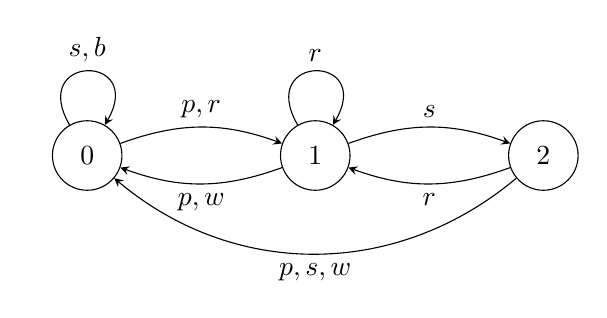
\begin{tikzpicture}[node/.style={draw, circle, inner sep=6pt}]
          \node[node] (0) {$0$};
          \node[node, right = 2cm of 0] (1) {$1$};
          \node[node, right = 2cm of 1] (2) {$2$};
    
          \path[->, >=stealth]
            (0) edge[loop above, in=60, out=120, looseness=6] node{$s, b$} (0)
            (0) edge[above, bend left = 20] node{$p, r$} (1)
            (1) edge[loop above, in=60, out=120, looseness=6] node{$r$} (1)
            (1) edge[below, bend left = 20] node{$p, w$} (0)
            (1) edge[above, bend left = 20] node{$s$} (2)
            (2) edge[below, bend left = 20] node{$r$} (1)
            (2) edge[below, bend left = 40] node{$p, s, w$} (0); 
        \end{tikzpicture}
      \end{center}
      \caption{精神状態の遷移図.それぞれのノードから$p,s,w,r$の4つの経路が出ていることを確認せよ.}
      \label{life_state}
\end{figure}

\begin{rei}{モナド}{monad}
    哲学において,このような考えは物の本性を考える上で大きな役割を果たしてきた.例えば『モナドロジー』においてライプニッツは,モナドを「非物体的なオートマトン(des Automates incorporels)」と呼び,アリストテレス的なエンテレケイアと同一視している.
    というのもライプニッツにとって,モナドとは固有の行動原理・プログラムを内部に持ち,それを展開していく存在にほかならないからだ.
    つまりモナドとは,一個のモノイドとして規定できる.
\end{rei} 


\begin{rei}{目的論的システム}{teleology}
    アリストテレスは,それぞれの事物は固有の運動原理を有すると考えた.
    例えば重いもの(土の元素を持つもの)はその本性から,下に向かう傾向がある.このように事物の本性から生じる運動は,自然的(natural)と言われる.
    一方,他の事物から力を受けて生じる運動(例えば上に投げられる等)は,強制的(forced)と言われる.
    事物固有の本性から生じる自然的運動は決まった方向性と到達点(telos)を持ち,その場所において,その事物は(他の強制力を受けない限り)運動をやめる.
    例えば重いものの到達点は地球の中心であり,そこに到達すると運動をやめる.逆に,他のものに妨げられない限り,それは中心へと向かい続ける(図\ref{fig:teleology}).
    
    このようにアリストテレスは,事物の状態(アリストテレスにとって,物理的事物の状態とは位置である)に働く作用は,自然力/強制力の2種に分別されると考えた.
    つまり,作用するモノイド$M$の元には自然$(N)$/強制$(F)$の2種類があり,何が自然とみなされるかは個物の本性によって決まってくるということだ.
    (本講では扱ってないが,このとき,$N, F$は$M$の部分モノイドとなる.)
    そして自然なモノイド作用は,事物をその「本来の場所」である到達点に運んでいく.こうした到達点を\emph{アトラクター}(attractor)という.
    到達点は,それ以上の自然モノイド作用によって変化しないという意味で,$N$の\emph{不動点}(fixed point)になっている.
    つまり目的とは自然モノイド作用のアトラクター/不動点である.    
\end{rei}

\begin{figure}[t]
    \begin{center}
        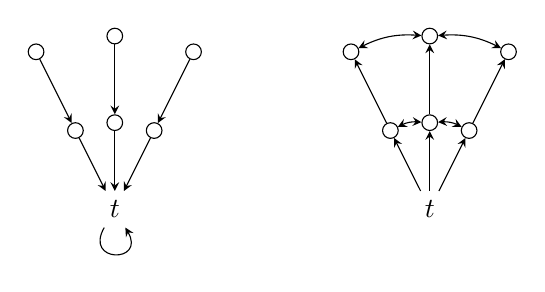
\begin{tikzpicture}[node/.style={draw, circle, inner sep=2pt}]
        \begin{scope} 
          \node (0) {$t$};
          \node[node] (10) at (-.5, 1) {};
          \node[node] (11) at (0, 1.1) {};
          \node[node] (12) at (.5, 1) {};
          \node[node] (20) at (-1, 2) {};
          \node[node] (21) at (0, 2.2) {};
          \node[node] (22) at (1, 2) {};
          (0) edge[loop below, in=60, out=120, looseness=6]  (0)
          \path[->, >=stealth]
            (21) edge (11)
            (11) edge (0)
            (20) edge (10)
            (10) edge (0)
            (22) edge (12)
            (12) edge (0)
            (0) edge[loop below, in=-60, out=-120, looseness=5]  (0);
        \end{scope} 
        \begin{scope}[xshift=4cm]
          \node (0) {$t$};
          \node[node] (10) at (-.5, 1) {};
          \node[node] (11) at (0, 1.1) {};
          \node[node] (12) at (.5, 1) {};
          \node[node] (20) at (-1, 2) {};
          \node[node] (21) at (0, 2.2) {};
          \node[node] (22) at (1, 2) {};
          \path[<-, >=stealth]
              (21) edge (11)
              (11) edge (0)
              (20) edge (10)
              (10) edge (0)
              (22) edge (12)
              (12) edge (0);
          \path[<->, >=stealth]
              (22) edge[above, bend right = 15] (21)
              (21) edge[above, bend right = 15] (20)
              (12) edge[above, bend right = 15] (11)
              (11) edge[above, bend right = 15] (10);
        \end{scope} 
        \end{tikzpicture}
      \end{center}
      \caption{アリストテレスによる,土の元素の自然運動(左)と強制運動(右).自然運動は地球の中心$t$にアトラクターを持つ.}
      \label{fig:teleology}
\end{figure}

上の事例において,個物の運動としてのモノイド作用が2種類に分けられるということ,そして自然モノイド作用が個物の本性によって定まるということは,アリストテレスの目的論的な運動論にとって本質的である(逆にアリストテレスにとって,個物の本性とはそうした自然モノイドそのものであると言えるかもしれない).
ガリレオ以降の近代物理学は,アリストテレスによるこうした運動の二類型を破棄することで築かれた.

\begin{rei}{決定論と非決定論}{indeterminism}
    2章で見た力学系を思い出そう.
    力学系では,系の状態$S$とその遷移関数$f:S \to S$の組み合わせによって,系の時間発展をモデル化するのだった.
    これは,一元$f$のみから生成されるモノイド$F$の$S$への作用として考えられる.
    つまり$F$に入るのは$f, f \circ f, f \circ f \circ f, \dots$など$f$を繰り返したもののみで,これによって任意のステップ先の状態が計算される.
    これを状態遷移図で書くと,すべてのノードからたった一つ(単位元$i$の作用を入れると二つ)の矢印のみが出ているものになる.
    すべての状態/ノードにおいて,次に遷移する先が一意に決まっているので,このシステムは決定論的である.
    
    それに対し,生成元が2元以上あるモノイドの作用は,非決定的な時間発展をモデル化している.
    実際,モノイド作用における異なる2元$m, n \in M$は,それぞれ異なった$S \to S$の関数を与える.
    この場合はノードからの矢印は複数になり,よって現在の状態からだけからは次の行き先が決まらない(どの作用が適用されるかにも依存する).
    これは人生モノイドを考えたとき,図\ref{fig:monoid_tree}のように人生が分岐していったことに合致している:つまり人生モノイドは我々が決定論に従わない,自由なエージェントであるということを仮定としている!
\end{rei}


\begin{renshu}{}{}
    モノイド作用もしくはオートマトンの例を挙げよ(自分で創作しても良い).
    その際,モノイド元と状態集合,および作用の積表を明示すること.
\end{renshu}
    

% チューリングマシンの例

% 最後にモノイド作用のもう一つ重要な適用例として,\emph{法則}の概念を取り上げよう.
% 法則とは,ある一定の系がどうふるまうかを規定するものである.
% そうだとすると,上で見てきたモノイド作用は,その作用対象である個物やエージェントが従う法則を表していると解釈することが可能である.
% しかしそれだけでなく,系として例えばある物理系をとれば,モノイド作用によってその物理系の時間的経過を表すことも可能だろう.
% このようなシステムを,一般に\emph{力学系}(dynamic systems)と呼ぶ.


% 我々が上で状態の集合としてきた集合$S$は,一般には\emph{状態空間}(state space)ないし相空間(phase space)と呼ばれる.
% モノイド作用は,



% このように考えると,モノイド作用の射程は極めて広く,時間発展する系一般を記述することができる.
% それには例えばコンピュータのプログラムの動作や,物理系の時間発展などが考えられる.
% 例えば古典力学の法則は,各質点の位置と運動量からなる\emph{状態空間}(state space)に対するモノイド作用として考えることができる.
% こうした時間発展系を\emph{力学系}(dynamic systems)という.

% \begin{rei}{決定論的世界観}
% \end{rei}


% この定義の集合$X$を$M$にすると,モノイドの定義2.1が復元されることを確認しよう.
% つまりすべてのモノイドは自分自身へのモノイド作用だといえる.\footnote{左作用についての注.}
% これまで見てきた「操作」としてのモノイドは,原則的にすべてこの「対象への作用」という面から捉え直すこともできる.
% 例えば足し算のモノイドでは,演算$+$は2つの整数(e.g., $5, 7$)をとって1つの整数($12$)を返す2項関数なのだった.
% しかし同様の事態を,全てのモノイド元$m$は,他のモノイド元$n$に「$m$を足す」1項関数,すなわち$m:M \to M, n \mapsto m+n$である,と表すこともできるだろう.
% これはつまり,例えば具体的な数7を,「7を足す」作用として考えよう,ということだ.
% モノイド元の合成は作用の合成,例えば$m+n$は「$m$を足してから$n$を足す」という一つの作用となり,また単位元$0$は「$0$を足す」(つまり何も変えない)という作用である.
% このようにモノイドは,「自分自身に働きそれを変える作用」として考えることができる.


% \begin{rei}{}{}
%     脳に加えられる外的・内的刺激全体を$M$とすると,$M$は脳状態へ作用するモノイドと捉えられる.ここで$m, n \in M$に対しその合成$mn$は,「刺激$m$を加えたあとに刺激$n$を加える」こととする(ただし「何も刺激を与えないこと」を単位元と考えるのは良くないかもしれない.その問題点を考えてみよ).
% \end{rei}








% \bibliographystyle{apalike}
% \bibliography{m4p}

\end{document}